%----------------------------------------------------------------------------------------
% Requisiti
%----------------------------------------------------------------------------------------

\documentclass[10pt]{softeng} % Document font size and equations flushed left

%----------------------------------------------------------------------------------------
%	DOCUMENT INFORMATION
%----------------------------------------------------------------------------------------


\Phase{Construction - I iterazione}


\DocumentTitle{Specifica dei Requisiti del Sistema} % Document title

%----------------------------------------------------------------------------------------

\begin{document}

\startofdocument{}

\section{Introduzione}

Si vuole realizzare un sistema di Home Banking (da ora HBS) per la gestione di fondi privati a breve, medio e lungo termine via Web. Il sistema è rivolto a Banche che decidono di implementare il protocollo/software Open Bank Project. Si presuppone che la banca già abbia uno stabile ed efficiente sistema di database di proprietà con opportuni software accessori, e in generale non si vuole analizzare la parte relativa al back-end della banca.  

Per rispettare e meglio implementare alcuni fondamentali requisiti non funzionali (sicurezza, tempi di reazione del sistema, ecc.), durante la stesura della proposta di progetto si è deciso di rimanere nell'ambito del \emph{retail banking}, ossia di progettare un sistema i cui unici utenti siano persone fisiche e non imprese o altri istituti finanziari.

Ogni individuo iscritto ad una banca possiede almeno un conto su cui depositare i propri risparmi: può essere \emph{di deposito} o \emph{corrente} a seconda che siano permesse le sole operazioni di prelievo e deposito o che in aggiunta a queste sia possibile  effettuare bonifici, pagamento di assegni, prelievi bancomat e simili.

\subsection{Utenti del sistema}

Gli utenti di questo sistema si dividono principalmente in due categorie: utenti registrati, o correntisti, e dipendenti della banca. 

Un individuo può ottenere un \emph{account HBS} in due passi:
\begin{enumerate}
	\item
	\begin{enumerate}
		\item se è già correntista della banca, gli basta fornire ad un dipendente della banca il proprio numero di conto;
		\item se non è correntista, deve compilare i moduli necessari all'apertura di un conto corrente (on-line o presso una filiale);
	\end{enumerate}
	\item in ogni caso, l'individuo deve recarsi in una filiale per consegnare copia di documento d'identità e ricevere le 					\emph{credenziali d'accesso} del proprio account.
\end{enumerate}

%TODO ?e se un correntista vuole aprire un altro conto?

Le funzionalità che verranno descritte nel seguito per gli \emph{account di servizio} e per gli \emph{account HBS} sono un nucleo identificato come necessario per soddisfare le necessit\`a di un generico sistema di Home Banking.
%Il \emph{pool} di progettisti e sviluppatori si impegna a implementare questo kernel nel modo più riutilizzabile e scalabile possibile, in modo da lasciare alla banca che adotti questo sistema la possibilità di operare come meglio crede con queste funzionalità, ad esempio creandone altre a partire da quelle qui elencate.

Un correntista deve poter:
\begin{itemize} 
	\item visionare \emph{saldo contabile annuale}, relativo all'anno in corso con eventuali grafici Valore/Tempo dell'andamento del valore rispetto agli anni precedenti;
	\item visionare \emph{saldo contabile mensile}, relativo al mese corrente con eventuali grafici Valore/Tempo dell'andamento del valore rispetto ai mesi precedenti;
	\item visionare \emph{saldo liquido} relativo al giorno corrente, nel caso in cui voglia compiere operazioni bancarie che coinvolgano calcolo di \emph{interesse};
	\item visionare \emph{saldo disponibile}, relativo al giorno corrente;
	\item visionare uno storico delle transazioni effettuate, avendo a disposizione per ogni transizione la \emph{data contabile}, l'\emph{importo versato} ed una \emph{causale};
	\item gestire operazioni periodiche o programmate;
	\item visionare informazioni delle carte di credito eventualmente collegate al conto;
	\item effettuare operazioni ``veloci'', inserendo pochi dati in una maschera preconfigurata e confermando l'operazione mediante meccanismo TOTP:
	\begin{itemize}
			\item ricariche telefoniche;
%			\item bonifici ordinari e bonifici SEPA mediante compilazione di opportuni moduli on-line;
			\item pagamento delle bollette;
	\end{itemize}
	\item visionare l'andamento in borsa dei titoli azionari del suo portafoglio;
	\item vendere uno o più titoli azionari del proprio portafoglio;
	\item investire il proprio patrimonio nei titoli di credito statali (NON azionari) a medio e lungo termine che ritiene più opportuni, avendo a disposizione un \emph{benchmark} per valutarne l'andamento in borsa e il profilo di rischio.
\end{itemize}	

Ad ogni account HBS è associato, oltre al conto corrente, un portafoglio azionario per conservare tutti i titoli bancari di cui il correntista sia in possesso.
Un portafoglio azionario ha un valore, calcolato in funzione dei valori di ogni azione contenuta al suo interno: modifiche di questo valore influiscono sul conto corrente associato al portafoglio, e il correntista non solo deve poter visionare tale valore e il suo andamento nel tempo, ma deve anche poter gestire il contenuto del portafoglio stesso.

I dipendenti della banca si dividono in \emph{impiegati} e \emph{dirigenti}. A ogni dipendente, sia esso impiegato o dirigente, viene assegnato un \emph{account di servizio}, con cui egli può assolvere alle sue mansioni specifiche; i vari account di servizio differiscono per permessi di accesso e funzionalità disponibili.

Ad ogni \emph{account di servizio} sono assegnati:
\begin{itemize}
	\item i dati del relativo dipendente;
	\item una password ``speciale'' (decidere politica di sicurezza).
\end{itemize}	

Gli \emph{impiegati}, mediante il loro account di servizio, devono poter: 
\begin{itemize}
	\item confermare/respingere atti che richiedono esplicita approvazione, ad esempio i bid per conti o carte inviati dagli utenti; 
	\item effettuare eventuali operazioni minori di contabilità e di gestione che una banca potrebbe permettere via internet.
\end{itemize}

I \emph{dirigenti} devono poter:
\begin{itemize}
	\item accedere e modificare i disclaimer pubblicitari del sito di home banking;
	\item impostare e modificare opportuni pacchetti di azioni o di fondi d'investimento e in generale offerte che si vogliono propinare agli utenti;
	\item selezionare, mediante opportuna combinazione di \emph{queries}, categorie o fasce di utenti in base a diversi parametri socio-economici, ed ottenere precise statistiche al riguardo;
	\item confermare atti di importanza superiore (a.e. alti investimenti in titoli azionari, transazioni di danaro molto elevate da un conto corrente ad un altro, ecc.), in seguito all'approvazione iniziale di un impiegato.
\end{itemize}

\subsection{Transazioni}

Una transazione economica è il passaggio sicuro e irreversibile da un conto ad un altro di una certa quantità di denaro.
La somma viene accreditata al \emph{conto destinatario} e detratta al \emph{conto mittente}, indipendentemente dalle banche di appartenenza, sfruttando ``indirizzi bancari'' come il codice IBAN.

%TODO cambiare in "bonifici programmati"
Sebbene non sia possibile annullare l'effetto di una transazione, l'utente pu\`o usufruire di funzionalit\`a di programmazione delle operazioni, sia essa una programmazione singola (``eseguire bonifico a tale beneficiario il tale giorno'') o una programmazione periodica (``eseguire un certo bonifico il tale giorno di ogni mese'', ad esempio per il pagamento di una rata).
L'utente pu\`o visualizzare e impostare tali transazioni programmate, e annullarle prima che vengano effettuate.

%Il nostro sistema vuole dare la possibilità alla banca che lo implementi di adottare una politica di ``conferma della transazione'': in uno scenario di e-commerce, una transazione tra un certo \emph{mittente} e un certo \emph{destinatario} viene confermata se il primo conferma di aver ricevuto in modo corretto il bene acquistato dal secondo, annullata se, viceversa, il primo è in grado di dimostrare la non corretta o avvenuta ricezione del bene acquistato.
%Per permettere questa funzionalità, si suddividerà la procedura di pagamento on-line in più step, ognuna delle quali avrà determinate peculiarità.

\subsection{Titoli di credito}

I titoli di credito sono, generalmente, strumenti finanziari mediante i quali i correntisti investono il proprio danaro: possono essere fondi comuni di investimento o azioni.
Ogni titolo di credito deve avere un \emph{benchmark}, calcolato dalla banca e visibile all'utente, che ne specifichi la \emph{volatilità} sul mercato.
Per motivi di sicurezza ed efficienza del sistema, si decide di non permettere l'acquisto diretto di titoli di credito su mercato nazionale e internazionale, ma di lasciare ad un account utente la possibilità di acquisire pacchetti preconfezionati dalla banca stessa.
Tuttavia ogni correntista può, attraverso il proprio account, avere delle dettagliate informazioni sull'andamento in borsa dei titoli che conserva nel suo portafoglio  e gli è lasciata la possibilità di vendere tali titoli nel caso lo ritenga opportuno.

\subsection{Bidding}

\`E possibile per un correntista o un individuo non registrato \emph{fare bidding}, ossia richiedere alla banca:
\begin{itemize}
	\item L'apertura di un conto corrente soggetto a condizioni specifiche.
	\item Il rilascio di una carta di credito soggetta a condizioni specifiche.
	\item La concessione di un mutuo/prestito a tasso e condizioni specifiche.
\end{itemize}

In base a delle regole definite dai dirigenti la proposta pu\`o essere:
\begin{itemize}
	\item approvata automaticamente dal sistema;
	\item inoltrata a un dipendente della banca per l'approvazione;
	\item rifiutata automaticamente.
\end{itemize}

Un possibile sistema di regole per l'approvazione dei bidding \`e l'individuazione di \emph{aree di risposta} basate sui parametri personalizzabili, come costo mensile di una carta di credito, tetto di spesa massima mensile, capacit\`a di prelievo allo sportello, etc.
Un esempio di come identificare queste aree di risposta \`e dato in figura \ref{fig:bidding}:
\begin{itemize}
	\item la zona compresa fra le linee tratteggiate verdi indica le condizioni (in questo caso una coppia di valori ``spesa massima mensile'' e ``costo mensile'' per una carta di credito) approvate automaticamente;
	\item la zona compresa fra le linee tratteggiate arancioni indica le condizioni soggette a verifica del dirigente della filiale prima dell'accettazione o del rifiuto;
	\item la zona compresa fra le linee tratteggiate rosse indica le condizioni rifiutate automaticamente.
		Le motivazioni di un rifiuto automatico possono essere differenti: un tetto di spesa mensile troppo alto a fronte di un costo mensile troppo basso potrebbe essere economicamente svantaggioso per la banca, mentre un tetto di spesa basso associato a un costo mensile alto potrebbe portare la banca a violare le normative vigenti a tutela dei suoi clienti.
\end{itemize}

\begin{figure}
	\resizebox{\columnwidth}{!}{
	\begin{tikzpicture}
		\begin{axis}[
			ymin=1,
			scale only axis,
			width=\columnwidth,
			ticks=none,
			domain=0:10,
			xlabel={Spesa massima mensile},
			ylabel={Costo mensile},
			axis lines=left,
			samples=200
        ]
		    \path[name path=axis] (axis cs:0,0) -- (axis cs:1,0);
		    \addplot[green] {x};
		    \addplot[green, dashed] {x-1};
		    \addplot[green, dashed] {x+1};
		    \addplot[orange, dashed] {x-2};
		    \addplot[orange, dashed] {x+2};
		    \addplot[red, dashed] {x-3};
		    \addplot[red, dashed] {x+3};
%   			\node [] at (axis cs:0.2,0) {basso};
%   			\node [] at (axis cs:0.6,0.3) {medio};
%   			\node [] at (axis cs:1.0,0.6) {alto};
%   			\node [] at (axis cs:1.4,1.2) {massimo};			
		\end{axis}
	\end{tikzpicture}
	}
	\caption{Un esempio di bidding: confronto fra spesa massima mensile di una carta di credito e costo di mantenimento della stessa.}
	\label{fig:bidding}
\end{figure}

Il sistema di bidding pu\`o portare diversi vantaggi alla banca che lo adotti:
\begin{itemize}
	\item fidelizzazione dell'utenza: un simile meccanismo permette alla banca di venire incontro alle esigenze di clienti di lunga data o con alta giacenza media mensile, che risultano essere ``buoni'' secondo le metriche della dirigenza, fornendo una possibilit\`a di interazione maggiore all'utente;
	\item contrasto della concorrenza: un cliente della banca potrebbe ricevere un'offerta conveniente da un istituto concorrente, ma scoprire autonomamente che un'offerta simile \`e disponibile anche presso la sua banca attuale;
	\item riduzione delle spese: automatizzando parte della ricerca dei contratti si riduce il carico di lavoro che i dipendenti della banca devono subire.
\end{itemize}

Un sistema di bidding presenta dei rischi, fra cui:
\begin{itemize}
	\item il sistema per stabilire i parametri di accettazione automatica potrebbe essere poco intuitivo e non fornire le metriche giuste, e il dirigente che se ne occupa viene portato a scelte che vanno contro gli interessi del suo istituto;
	\item il sistema di bidding potrebbe essere troppo complesso per l'utenza della banca e non venir utilizzato.
\end{itemize}
Tutti questi rischi devono essere gestiti correttamente durante lo sviluppo del sistema.

%TODO pubblicità contestuale on-demand di bidding?

\subsection{Home Trading}

HBS deve implementare una gestione (seppur parziale) dei portafogli fondi dei clienti della banca.

La soluzione individuata, chiamata \emph{Home Trading}, ha le seguenti caratteristiche:
\begin{itemize}
	\item La banca che sfrutta il sistema di \emph{Home Trading} confeziona \emph{pacchetti di investimento} contenenti un certo numero di titoli azionari.
	I pacchetti di investimento vengono proposti ai clienti della banca tramite HBS.
	\item I clienti possono visualizzare informazioni sull'andamento passato dei titoli azionari contenuti in un pacchetto di investimento, assieme a una valutazione del rischio effettuata dal dipendente responsabile del confezionamento del pacchetto.
	I clienti possono acquistare un pacchetto di investimento per un periodo di tempo predeterminato.
	\item A ogni pacchetto di investimento \`e associata una soglia minima (inferiore al prezzo di acquisto) di \emph{valore garantito} del pacchetto.
	Qualora un cliente di HBS voglia vendere un pacchetto di investimento prima del tempo predeterminato, ricever\`a dalla banca il valore garantito del pacchetto, indipendentemente dall'andamento delle azioni contenute nel pacchetto.
	\item Al termine del periodo di possesso del pacchetto i clienti di HBS ricevono dalla banca una somma commisurata alle perdite o ai guadagni delle azioni contenute nel pacchetto.
	Il valore del pacchetto non pu\`o scendere sotto il \emph{valore garantito} stabilito dalla banca, ossia in caso di perdita delle azioni contenute nel pacchetto la perdita del cliente che ha effettuato l'invesitmento \`e sempre minore o uguale alla differenza fra prezzo originale del pacchetto e valore garantito del pacchetto.
\end{itemize}

Il sistema di \emph{Home Trading} proposto permette di gestire i portafogli fondi dei clienti della banca, senza incorrere nell'elevata complessit\`a caratterizzante sistemi di \emph{trading} professionali.


\section{Glossario}
%(versione 1 : sono omesse definizioni banali e/o implicite)

\paragraph{Accoppiamento}
\`e il grado di dipendenza di una componente del sistema software dalle altre componenti.
L'accoppiamento \`e un fenomeno negativo in contrapposizione con la coesione.
Alto accoppiamento rende difficile la manutenzione e la modifica del codice.

\paragraph{Audit di sicurezza} 
	operazioni di controllo del sistema effettuate periodicamente per controllare che non ci siano sate violazioni della politica di sicurezza adottata
\paragraph{Banca D'Italia}
	 Banca centrale della Repubblica Italiana, avente funzione sia di vigilanza su banche, istituti di credito, intermediari finanziari sia di principale controllore in materia di antiriciclaggio: insieme alla CONSOB, deve avere libero accesso, entro i termini previsti dalla legge, ai dati contenuti nei database di qualsiasi istituto finanziario che operi sul territorio italiano. \cite{banca_italia}
\paragraph{Bonifico} \label{glossario:bonifico}
	operazione bancaria mediante la quale si mette a disposizione di una persona o le si accredita una somma di denaro per ordine e conto di altri
\paragraph{Bonifico SEPA} \label{glossario:bonifico-sepa}
	bonifico (v.~\hyperref[glossario:bonifico]{bonifico}) accreditabile ad un destinatario ubicato oltre i confini nazionali nell'area \hyperref[glossario:sepa]{SEPA}.
\paragraph{Codice IBAN}
	L'International Bank Account Number è uno standard internazionale utilizzato per identificare un'utenza bancaria e/o operazione associata ad un conto corrente 
\paragraph{Codice BIC/SWIFT}
	standard che definisce i \emph{bank identifier codes} (codici d'identificazione bancaria) approvato dall'International Organization for Standardization (ISO). Questi codici vengono utilizzati per i trasferimenti di denaro tra banche, specialmente nelle transazioni internazionali, per le quali è spesso ancora necessario nonostante l'entrata in vigore dell'IBAN. \cite{bic_wiki}
\paragraph{Commissione Nazionale per le societ\`a e la borsa (CONSOB)}
	è un'autorità amministrativa indipendente, dotata di personalità giuridica e piena autonomia la cui attività è rivolta alla tutela degli investitori, all'efficienza, alla trasparenza e allo sviluppo del mercato mobiliare italiano. \cite{consob_wiki}
\paragraph{Conto Corrente (cc)}
indica un deposito di danaro effettuato dal possesore del bene, detto \emph{correntista}, in una banca o istituto di credito
\paragraph{Correntista} \label{glossario:correntista}
	persona fisica o giuridica titolare di un Conto Corrente presso la banca utente di HBS.
\paragraph{Downtime}
termine inglese per rappresentare il tempo di fermo di un sistema informatico.
Puo essere dovuto alla manutenzione programmata oppure al malfunzionamento.
Opposto di Uptime.
\paragraph{Fondo comune di investimento}
	è un istituto d'intermediazione finanziaria mediante il quale è possibile partecipare, investita una determinata quota di danaro, alla gestione e alla spartizione di dividendi prodotti da un determinato \emph{bene mobiliare} nel tempo. La \emph{banca depositaria} ne custodisce materialmente i titoli e ne tiene in cassa le disponibilità liquide. Le banche hanno inoltre un ruolo di controllo sulla legittimità delle attività del fondo sulla base di quanto prescritto dalle norme della Banca d'Italia e dal regolamento del fondo stesso
\paragraph{Istituto di credito}
	organismo che svolge simultaneamente l’attività di raccolta di risorse finanziarie e di concessione del credito per proprio contoa terzi 
\paragraph{Microservizio}
unit\`a software indipendente progettata per svolgere un singolo compito specifico. Insieme pi\`u microservizi formano un sistema modulare a basso accoppiamento. In un sistema orientato a microservizi un modulo \`e facilmente rimpiazzabile senza compromettere la funzionalit\`a del sistema.

\paragraph{Open Bank Project (OBP)}
	è una API open source che permette a banche ed istituti di credito di creare un interfaccia utente di ampia portata e fruibilità. Essendo un sistema molto versatile e largamente riadattabile, si presta molto a definire un vero e proprio \emph{standard di interfaccia}, ossia a definire un canone per la creazione di interfacce rivolte e all'utenza bancaria generica e agli organismi deputati al controllo bancario. \cite{obp}
\paragraph{Portafoglio valori/titoli azionari}
	è l'insieme dei diversi titoli finanziari e/o fondi d'investimento che l'utente bancario generico può possedere.Ogni titolo e/o fondo acquisito viene inserito nel portafoglio.
\paragraph{Refactoring}
	processo di riutilizzazzione di codice già scritto in precedenza, senza doverne generare di nuovo
\paragraph{Saldo attuale} \label{glossario:saldo-attuale}
	\`e la somma algebrica di tutte le operazioni avvenute sul conto (entrate e uscite) e registrate sul conto ad una certa data.
\paragraph{Saldo contabile} \label{glossario:saldo-contabile}
	è il saldo totale effettivamente a disposizione e tiene conto in positivo di eventuali fidi ed in negativo di assegni versati ma non ancora disponibili.
	Indica quanto effettivamente \`e presente sul conto e di cui il correntista pu\`o disporre per prelevare, effettuare pagamenti, bonifici ecc.
\paragraph{Saldo liquido} \label{glossario:saldo-liquido}
	\`e la somma disponibile su cui vengono calcolati gli interessi.
\paragraph{SEPA} \label{glossario:sepa}
	La SEPA (Single Euro Payments Area) è l’area unica in cui i cittadini, le imprese e gli enti, possono eseguire e ricevere pagamenti in Euro, all’interno dei confini nazionali e tra i paesi diversi che compongono l’area SEPA con condizioni di base, diritti ed obblighi uniformi tra i paesi stessi. 
\paragraph{Time-based One Time Password (TOTP)}
	è un algoritmo che calcola una \emph{One-Time password} combinando mediante una funzione hash una chiave segreta condivisa ed il tempo corrente. \cite{totprfc}
\paragraph{TLS - Transport Layer Security}
Un protocollo di comunicazione sicura. Usa gli algoritmi di crittografia per garantire una comunicazione sicura fra due terminali informatici su una rete che usa il protocollo tcp/ip.
Garantisce inoltre l'autenticit\`a e l'integrit\`a dei messaggi trasmessi.
Conosciuto anche come SSL.
\paragraph{Trading online}
	pratica uguale a quella del \emph{trading} bancario classico mediante aiuto di personalità con competenze specifiche(v.broker), effettuata però in rete, disponendo cioè di opportuni strumenti software per il monitoraggio di mercati azionari nazionali e internazionali e  per il controllo completo e \emph{real time} del proprio portafoglio azionario.
\paragraph{Uptime}
    termine inglese che denota il tempo in cui il sistema informatico \`e attivo e funziona correttamente.
    Opposto di Downtime.


\paragraph{VPN - Virtual Private Network}
        \`e una tecnologia per estendere una rete informatica privata, sfruttando come strato sottostante una rete publica.
    Definisce una serie di protocolli di comunicazione e crittografia che permettono la comunicazione sicura ed affidabile.
    Una VPN permette di avere gli stessi vantaggi di una linea privata, ma a un costo significativamente inferiore.
\subsection{Virtualizzazione}
\paragraph{Virtualizzazione dell'hardware}
\`e una tecnologia dove il sistema operativo non viene eseguito direttamente su una macchina fisica, ma viene creata una macchina virtuale che emula il comportamento della macchina fisica. In genere il sistema operativo e i processi che girano sulla macchina virtuale non sono influenzati dai processi esterni alla macchina virtuale, ma possono comunicare.
Usando questo approccio le componenti hardware vengono emulate in software, introducendo overhead.
Questo approccio offre molti vantaggi come flessibilit\`a e indipendenza dalla piattaforma.
\paragraph{Virtualizzazione al livello del sistema operativo}
\`e una tecnologia dove il kernel del sistema operativo viene eseguito sulla macchina fisica. Il software di virtualizzazione \`e una parte del kernel. I processi vengono eseguiti all'interno dei container, che sono isolati fra loro, e non possono interferire con i processi negli altri container. I container tuttavia possono essere configurati per permettere la comunicazione.
Ogni processo viene esegito direttamente sulla CPU fisica della macchina, e l'hardware non viene emulato.
In genere la virtualizzazione al livello del sistema operativo ha performance migliori rispetto alla virtualizzazione hardware.




\section{Definizione dei Requisiti Utente}

Di seguito \`e illustrata la descrizione dettagliata dei requisiti utente.

\subsection{Requisiti Funzionali}
\label{sec:utente:funzionali}

I requisiti funzionali individuati per il sistema HBS sono i seguenti:

\begin{enumerate}
	\item \label{itm:utente:funzionali:iscrizione} Ogni utente correntista che ne faccia esplicita richiesta deve avere un account personale e deve potersi iscrivere  mediante apposite procedure (business case in figura \ref{fig:business_case_registration}).
	\item \label{itm:utente:funzionali:gestione-conto} Un utente registrato deve poter effettuare l'amministrazione corretta del proprio conto corrente (business case in figura \ref{fig:business_case_generic_operation}), per questa ragione è richiesto che:
	\begin{enumerate}
		\item \label{itm:utente:funzionali:gestione-conto:verifica-saldo} l'utente possa verificare in tempo reale:
			\begin{itemize}
				\item il suo saldo attuale;
				\item il suo saldo contabile;
				\item il suo saldo liquido;
			\end{itemize}
		\item \label{itm:utente:funzionali:gestione-conto:verifica-andamento} l'utente deve poter verificare in tempo reale l'andamento dei titoli azionari che possiede e, eventualmente, venderli;
		% \item \label{itm:utente:funzionali:gestione-conto:revisione} l'utente deve poter effettuare operazioni programmate di revisione dei conti o di pagamento;
		\item \label{itm:utente:funzionali:gestione-conto:operazioni} l'utente deve poter effettuare disposizioni generiche di pagamento;
		\item \label{itm:utente:funzionali:gestione-conto:operazioni-veloci} l'utente deve poter effettuare \emph{operazioni veloci}, ossia effettuare disposizioni inserendo pochi dati in una maschera preconfigurata, come:
			\begin{itemize}
				\item ricariche telefoniche;
				\item bonifici ordinari;
				\item bonifici SEPA;
				\item pagamento delle bollette.
			\end{itemize}
	\end{enumerate}
	\item \label{itm:utente:funzionali:storico} L'utente deve poter consultare lo storico delle transazioni eseguite, complete delle informazioni riguardanti la data, il destinatario, l'importo previsto e una causale descrittiva delle motivazioni;
	% \item \label{itm:utente:funzionali:resoconto} L'utente deve poter ottenere, in tempo reale, un resoconto delle transazioni che sono in corso da e verso il suo conto;
	\item \label{itm:utente:funzionali:dipendenti:accesso} I dipendenti di una banca, impiegati e manager, devono poter accedere al sistema mediante specifico e personale account;
	\item \label{itm:utente:funzionali:dipendenti:operazioni-veloci} I dipendenti di una banca devono poter creare i form per la gestione delle operazioni veloci;
	\item \label{itm:utente:funzionali:management:bidding:approvazione} I manager devono poter accettare o rifiutare le proposte di bidding per conti correnti, carte di credito e prestiti fatte dagli utenti che rientrano nell'insieme di proposte soggette a approvazione dei manager della banca.
	\item \label{itm:utente:funzionali:management:bidding:creazione} I manager devono poter gestire il bidding eventualmente offerto della banca, specificando in modo opportuno per conti correnti, carte di credito e prestiti i parametri che individuano i bid accettati automaticamente, soggetti a ulteriore approvazione, rifiutati automaticamente.
	I parametri di decisione comprendono i parametri di conti correnti, carte di credito e prestiti, e parametri riguardanti i clienti della banca.
	Alcuni possibili parametri sono:
		\begin{itemize}
			\item giacenza media mensile e annuale sui conti correnti dell'utente;
			\item affidibilit\`a dell'utente (in funzione, ad esempio, della frequenza con cui i suoi conti correnti sono andati in rosso);
			\item da quanto tempo il correntista \`e cliente presso la banca;
			\item eventuali altri parametri.
		\end{itemize}
	\item \label{itm:utente:funzionali:management:pacchetti-investimento:creazione} I manager devono poter creare \emph{pacchetti di investimento}.
		Un pacchetto di investimento contiene titoli azionari prelevati da un \emph{pool} di azioni acquistate dalla banca.
		Il pacchetto di investimento deve contenere le seguenti informazioni:
		\begin{itemize}
			\item andamento passato dei titoli contenuti nel pacchetto;
			\item valutazione di rischio prodotta dal manager che ha creato il pacchetto;
			\item costo del pacchetto;
			\item valore garantito di vendita del pacchetto;
			\item percentuale di guadagno della banca alla vendita del pacchetto.
		\end{itemize}
		I pacchetti di investimento vengono acquistati dai clienti della banca e formano un \emph{portafoglio di investimento}.
	\item \label{itm:utente:funzionali:management:pubblicita} I manager devono poter gestire in modo efficiente gli spazi pubblicitari offerti dalle pagine web del sistema, potendone arbitrariamente modificare i contenuti e indirizzando determinate pubblicità ad determinati insiemi di utenti aventi delle caratteristiche desiderate.
	\item \label{itm:utente:funzionali:notifiche} Il sistema HBS deve inviare ad ogni utente una notifica tramite SMS o e-mail (a scelta dell'utente) a seguito di ogni operazione tra le seguenti:
		\begin{itemize}
			\item ogni volta che si conclude una transazione da o verso il proprio conto corrente;
			\item ad ogni login e logout dall'account HBS;
			\item ad ogni \emph{operazione veloce} di pagamento.
		\end{itemize}
	Ogni notifica \`e abilitabile o disabilitabile singolarmente secondo le preferenze dell'utente.
	\item \label{itm:utente:funzionali:storico-dettagliato} Il sistema di Home Banking deve fornire ai suoi utenti (clienti della banca, dipendenti della banca, agenti di terze parti) la possibilit\`a di visualizzare uno storico dettagliato di ogni operazione (requisito funzionale) effettuata seguendo un opportuno sistema di privilegi.
\end{enumerate}

\subsection{Requisiti Non Funzionali}
\label{sec:utente:non-funzionali}

\begin{enumerate}
	\item \label{itm:utente:non-funzionali:logging} Ogni operazione effettuata da un utente (cliente della banca o dipendente della banca) sul sistema deve essere registrata in un log.
	Ogni log deve contenere quantomeno le seguenti informazioni:
	\begin{itemize}
		\item un'identificativo del tipo di operazione eseguita;
		\item il conto coinvolto nell'operazione;
		\item l'istante dell'operazione;
		\item informazioni riguardanti il terminale da cui \`e stata effettuata l'operazione.
	\end{itemize}

	\item \label{itm:utente:non-funzionali:uptime} Il sistema di Home Banking ha dei requisiti impliciti di disponibilit\`a, ovvero il sistema deve avere una percentuale minima garantita di \emph{uptime}, o tempo in cui il sistema \`e disponibile e utilizzabile dagli utenti.

	La percentuale di \emph{uptime} non comprende eventuale tempo di \emph{downtime} previsto periodicamente per motivi di manutenzione, ottimizzazione delle prestazioni, aggiornamento, etc.

	Le percentuali di \emph{uptime} garantito e di \emph{downtime} richiesto devono essere definite in funzione della quantit\`a di operazioni gestita dal sistema, ossia in funzione del numero di utenti attivi presso un particolare istituto bancario e della mole di transazioni effettuate quotidianamente, e in funzione delle caratteristiche delle macchine su cui il software viene installato presso un particolare istituto bancario.

	La percentuale di \emph{uptime} garantito e di \emph{downtime} richiesto deve quindi essere stabilita e personalizzata al momento della vendita del software ad un istituto bancario.

	\item \label{itm:utente:non-funzionali:usabilita} Il sistema di Home Banking ha dei requisiti impliciti di usabilit\`a, ovvero:
	\begin{enumerate}
		\item \label{itm:utente:non-funzionali:usabilita:clienti} deve essere utilizzabile senza particolare addestramento dai clienti della banca;
		\item \label{itm:utente:non-funzionali:usabilita:management} deve essere utilizzabile dopo addestramento minimo dai dipendenti della banca.
	\end{enumerate}
	Le operazioni disponibili per i clienti della banca (requisiti funzionali) devono essere facilmente utilizzabili e comprensibili.
	Ogni maschera per l'inserimento di informazioni deve essere corredata da opportuni testi brevi illustranti il tipo di informazioni richieste.
\end{enumerate}

\subsubsection{Requisiti di Sicurezza del Sistema}
\label{sec:utente:non-funzionali:sicurezza}

Il sistema di Home Banking presenta forti requisiti non funzionali di sicurezza.

\begin{enumerate}
	\item \label{itm:utente:non-funzionali:sicurezza:accesso} L'accesso al sistema di Home Banking da parte di un utente avviene a seguito di autenticazione dello stesso.
		Le credenziali di accesso devono essere trasmesse dal browser dell'utente al sistema di Home Banking utilizzando una connessione sicura.
	\item \label{itm:utente:non-funzionali:sicurezza:credenziali} Le credenziali d'accesso per un account sono:
		\begin{itemize}
			\item numero conto corrente;
			\item password fornita al correntista al momento della registrazione.
		\end{itemize}
	\item \label{itm:utente:non-funzionali:sicurezza:operazioni} Le operazioni effettuabili dall'utente (requisiti funzionali) sono partizionate in operazioni che richiedono un'ulteriore autenticazione tramite One Time Password e operazioni che \emph{non} richiedono ulteriore autenticazione.
	Ogni operazione \`e eseguibile solo dopo che l'utente ha effettuato l'accesso al sistema di Home Banking.

	Le seguenti operazioni non richiedono ulteriore autenticazione:
	\begin{itemize}
		\item visionare saldo contabile, disponibile e liquido;
		\item visionare uno storico delle transazioni effettuate;
		\item visionare informazioni riguardo le carte di credito collegate al conto (se presenti);
		\item effettuare ``operazioni veloci'' impostate attraverso un sistema di configurazione.
	\end{itemize}

	Ogni altra operazione richiede autenticazione tramite One Time Password.
	In particolare \`e richiesta autenticazione tramite One Time Password per:
	\begin{itemize}
		\item effettuare transazioni, come:
		\begin{itemize}
			\item bonifici ordinari, bonifici SEPA;
			\item ricariche carte prepatate e schede telefoniche;
			\item pagamento bollette, bollettini, tasse, etc;
			\item modificare le preferenze dell'utente, come frequenza delle notifiche, etc.
		\end{itemize}
		\item configurare operazioni veloci.
	\end{itemize}
\end{enumerate}

\subsection{Requisiti di Dominio}
\label{sec:utente:dominio}

La legislazione attuale richiede che gli organi di controllo finanziario come la Banca d'Italia e le forze dell'ordine possano accedere in lettura a tutte le informazioni salvate dal sistema di Online Banking.

\begin{enumerate}
	\item \label{itm:utente:dominio:vpn} Ogni sistema informatico nell'ambito bancario, e in particolare il software HBS in sviluppo, deve permettere l'accesso da remoto alla sua rete interna tramite il meccanismo di \emph{VPN}.
	HBS deve quindi fornire alle autorit\`a di controllo le credenziali e/o interfacce per accedere ai sistemi di \emph{data storage}.

	\item \label{itm:utente:dominio:forze-ordine} Le forze dell'ordine, dato un utente, devono poter visualizzare le seguenti informazioni:
        \begin{enumerate}
           	\item tutte le transazioni effettuati dall'utente;
            \item tutte le transazioni che hanno l'utente come destinatario;
	        \item dati anagrafici dell'utente;
    	    \item informazioni riguardo al terminale informatico dal quale l'\emph{account} dell'utente \`e stato acceduto in precedenza.
		\end{enumerate}
		In caso le informazioni siano ridondanti il sistema deve fornire alle ff. oo. un modo per confrontare le informazioni e fare il controllo di coerenza.
%TODO da qualche parte bisogna dire che un haxxor in genere non puo modificare tutti i log in maniera coerente, perche pensa a rubare i dindi invece di giocare ad uplink

	\item \label{itm:utente:dominio:controllo-finanziario} L'organo di controllo finanziario, dato un utente, deve poter visualizzare le seguenti informazioni:
        	\begin{enumerate}
	            \item tutte le transazioni effettuate dall'utente;
    	        \item tutte le transazioni che hanno l'utente come destinatario;
	            \item lo storico di Online Trading dell'utente.
    	    \end{enumerate}
	La normativa legale richiede che un sistema in grado di offrire funzionalit\`a di trading fornisca all'organo di controllo finanziario l'accesso allo storico delle operazioni, in particolare l'organo di controllo deve poter:
	\begin{enumerate}
    	\item visualizzare le informazioni dei pacchetti di Online Trading;
    	\item visualizzre lo storico del sistema di Online Trading.
    	%TODO non so se ci va visualizzare mutui e tassi
	\end{enumerate}

	\item \label{itm:utente:dominio:controllo-finanziario:bidding} Poich\'e il sistema di Bidding deve rispettare le normative legali, per esempio le leggi sull'usura bancaria, l'ente responsabile del controllo finanziario deve poter:
	\begin{enumerate}
    	\item accedere allo storico del sistema Bidding;
    	\item visualizzare i parametri entro i quali le proposte vengono accettate automaticamente;
    	\item visualizzare informazioni delle proposte accettate dal management;
    	\item visualizzare proposte negate dal management.
	\end{enumerate}

\end{enumerate}

%TODO conti sono observable, la gg.ff. puo definire trigger. .. . \ldots .. \ldots \ldots eas\ldots \ldots .. \ldots \ldots ..



\section{Specifica dei Requisiti di Sistema}

Di seguito \`e esposta la specifica dei requisiti di sistema.

Ciascun requisito \`e specificato su una scheda seguendo l'esempio illustrato da \cite[p. 97]{sommerville}.
In particolare ciascuna scheda conterr\`a i seguenti campi:
\begin{itemize}
	\item ID del requisito;
	\item tipo del requisito;
	\item titolo del requisito;
	\item descrizione del requisito;
	\item origine del requisito;
	\item priorit\`a del requisito.
\end{itemize}
I requisiti funzionali conterranno inoltre i seguenti campi:
\begin{itemize}
	\item input del requisito funzionale;
%	\item origine dell'input;
	\item output del requisito funzionale;
%	\item destinazione dell'output;
	\item descrizione dell'azione.
%	\item pre-condizioni;
%	\item post-condizioni;
%	\item side-effects.
\end{itemize}

Identifichiamo i requisiti del sistema con la codifica ottenuta concatenando i seguenti elementi, usando un \emph{underscore} come separatore:
\begin{itemize}
	\item il prefisso comune \code{REQ};
	\item una sequenza di 4-10 lettere (identificativo mnemonico);
	\item un identificativo di priorit\`a (in ordine decrescente \code{A}, \code{M}, \code{B});
	\item un identificativo della tipologia (\code{F} per requisiti funzionali, \code{N} per requisiti non funzionali, \code{D} per requisiti di dominio);
	\item un intero strettamente positivo (unico per ogni requisito, per ogni tipologia).
\end{itemize}
In contesti in cui \`e necessario essere concisi \`e possibile identificare i requisiti utilizzando unicamente il prefisso \code{REQ}, la tipologia del requisito e l'intero assegnato al requisito.

\def\idDISPAG{REQ\_DISPAG\_F\_A\_1\,}
\def\shortidDISPAG{REQ\_F\_1\,}

\def\idISCRCORR{REQ\_ISCRCORR\_F\_A\_2\,}
\def\shortidISCRCORR{REQ\_F\_2\,}

\def\idCROPVEL{REQ\_CROPVEL\_F\_M\_3\,}
\def\shortidCROPVEL{REQ\_F\_3\,}

\def\idSECAUTH{REQ\_SECAUTH\_N\_A\_1\,}
\def\shortidSECAUTH{REQ\_N\_1\,}

\def\idDISOPVEL{REQ\_DISOPVEL\_F\_M\_4\,}
\def\shortidDISOPVEL{REQ\_F\_4\,}

\def\idAPPBID{REQ\_APPBID\_F\_M\_5\,}
\def\shortidAPPBID{REQ\_F\_5\,}

\def\idVERSAL{REQ\_VERSAL\_F\_A\_6\,}
\def\shortidVERSAL{REQ\_F\_6\,}

\def\idVERTIT{REQ\_VERTIT\_F\_M\_7\,}
\def\shortidVERTIT{REQ\_F\_7\,}

\def\idDIPACC{REQ\_DIPACC\_F\_A\_8\,}
\def\shortidDIPACC{REQ\_F\_8\,}

\def\idLOGOP{REQ\_LOGOP\_N\_A\_2\,}
\def\shortidLOGOP{REQ\_N\_2\,}

\def\idVERSTOR{REQ\_VERSTOR\_F\_A\_9\,}
\def\shortidVERSTOR{REQ\_F\_9\,}



\subsection{Specifica dei Requisiti Funzionali}

\subsubsection{\code{REQ\_F\_1} - Disposizioni di Pagamento}
\label{sec:sistema:funzionali:DISPAG}

\begin{ptable}{3}
\ptitlerow{Titolo}
\prow{
		Disposizioni di Pagamento
}
\pline
\pcells{ID & Tipologia & Priorit\`a}
\pcells{
	$\code{REQ\_DISPAG\_F\_A\_1}$ & Funzionale & Alta
}
\pline
\ptitlerow{Descrizione requisito}
\prow{
		Un utente registrato al sistema di Home Banking deve poter effettuare generiche disposizioni di pagamento. In particolare l'utente deve poter effettuare bonifici (p.~\pageref{glossario:bonifico}) e bonifici SEPA (p.~\pageref{glossario:bonifico-sepa}).
}
\pline
\ptitlerow{Origine requisito}
\prow{
		Requisiti utente (sez.\ \ref{sec:utente:funzionali}, req.\ \ref{itm:utente:funzionali:gestione-conto:operazioni}).
}
\pline
\ptitle{Input}
\pcell{1}{
		Numero di conto corrente, tipologia dell'operazione, somma di denaro da trasferire, conto corrente di destinazione nel formato opportuno.
}
\pline
\ptitle{Output}
\pcell{1}{
		Indicatore di successo dell'operazione.
}
\pline
\ptitlerow{Descrizione azione}
\prow{
		L'operazione specificata viene inoltrata da HBS al back-end della banca. HBS attende dal back-end informazioni riguardo il successo o meno dell'operazione.
}
%\pline
%\ptitlerow{Pre-condizioni}
%\prow{
%		L'utente ha accesso al conto corrente indicato. Il saldo contabile sul conto corrente indicato \`e maggiore o uguale alla somma di denaro da trasferire pi\`u eventuali spese di commissione.
%}
%\pline
%\ptitlerow{Post-condizioni}
%\prow{
%		Se il back-end della banca ha preso in carico l'operazione con successo, la gestione della stessa \`e stata passata al back-end. Altrimenti nessuna.
%}
%\pline
%\ptitlerow{Side-effects}
%\prow{
%		Il tentativo di operazione viene registrato nel log di HBS, insieme ad informazioni riguardo lo stato di presa in carico da parte del back-end della banca.
%}
\end{ptable}

\subsubsection{\code{REQ\_F\_2} - Iscrizione Nuovo Correntista}
\label{sec:sistema:funzionali:ISCRCORR}

\begin{ptable}{3}
\ptitlerow{Titolo}
\prow{
		Iscrizione Nuovo Correntista
}
\pline
\pcells{ID & Tipologia & Priorit\`a}
\pcells{
	$\code{REQ\_ISCRCORR\_F\_A\_2}$ & Funzionale & Alta
}
\pline
\ptitlerow{Descrizione requisito}
\prow{
		Il sistema deve permettere l'iscrizione a correntisti (p.~\pageref{glossario:correntista}) che non possiedano gi\`a un account HBS tramite un form compilabile e inviabile via web-browser.
}
\pline
\ptitlerow{Origine requisito}
\prow{
		Requisiti utente (sez.\ \ref{sec:utente:funzionali}, req.\ \ref{itm:utente:funzionali:iscrizione}).
}
\pline
\ptitle{Input}
\pcell{1}{
		Numero di conto corrente e codice fiscale del correntista.
}
\pline
\ptitle{Output}
\pcell{1}{
		Indicatore di avvenuta presa in carico della richiesta di iscrizione da parte del sistema di HBS.
}
\pline
\ptitlerow{Descrizione azione}
\prow{
		La richiesta di iscrizione viene presa in carico dal sistema e inserita nel database di HBS.
}
%\pline
%\ptitlerow{Pre-condizioni}
%\prow{
%		Il numero di conto corrente corrisponde a un conto corrente registrato presso l'istituto in questione. Il codice fiscale corrisponde alla persona fisica o giuridica cui il conto corrente \`e intestato. Non esiste un utente HBS associato al codice fiscale del correntista.
%}
%\pline
%\ptitlerow{Post-condizioni}
%\prow{
%		Viene creato un utente HBS associato al codice fiscale del correntista. Il nuovo utente non \`e abilitato all'accesso a HBS (v.\ requisiti \ref{itm:utente:funzionali:approvazione}). Il conto corrente associato al numero di conto corrente inserito viene abilitato all'uso di HBS.
%}
%\pline
%\ptitlerow{Side-effects}
%\prow{
%		La richiesta di iscrizione viene inserita nel database di HBS.
%}
\end{ptable}

\subsubsection{\code{REQ\_F\_3} - Creazione Operazioni Veloci}
\label{sec:sistema:funzionali:CROPVEL}

\begin{ptable}{3}
\ptitlerow{Titolo}
\prow{
		Creazione Operazioni Veloci
}
\pline
\pcells{ID & Tipologia & Priorit\`a}
\pcells{
	$\code{REQ\_CROPVEL\_F\_M\_3}$ & Funzionale & Media
}
\pline
\ptitlerow{Descrizione requisito}
\prow{
		I dipendenti della banca devono poter definire operazioni veloci utilizzabili dai clienti della stessa. Un'operazione veloce permette di effettuare operazioni ordinarie quali bonifici (p.~\pageref{glossario:bonifico}) o bonifici SEPA (p.~\pageref{glossario:bonifico-sepa}) inserendo un numero ridotto di argomenti rispetto a quelli normalmente necessari. Vedi anche requisito funzionale \ref{itm:utente:funzionali:gestione-conto:operazioni-veloci}.
}
\pline
\ptitlerow{Origine requisito}
\prow{
		Requisiti funzionali (sez.\ \ref{sec:utente:funzionali}, req.\ \ref{itm:utente:funzionali:dipendenti:operazioni-veloci}).
}
\pline
\ptitle{Input}
\pcell{1}{
		Nome dell'operazione veloce, parametri dell'operazione veloce, operazione tradizionale corrispondente, mapping dei parametri dell'operazione veloce nei parametri dell'operazione tradizionale.
}
\pline
\ptitle{Output}
\pcell{1}{
		Informazioni riguardo il successo dell'inserimento dell'operazione veloce nel database di HBS.
}
\pline
\ptitlerow{Descrizione azione}
\prow{
		Le informazioni fornite vengono inserite nel database di HBS contenente le informazioni sulle operazioni veloci configurate dalla banca.
}
%\pline
%\ptitlerow{Pre-condizioni}
%\prow{
%		Precondizioni.
%}
%\pline
%\ptitlerow{Post-condizioni}
%\prow{
%		Postcondizioni.
%}
%\pline
%\ptitlerow{Side-effects}
%\prow{
%		Side effects.
%}
\end{ptable}

\subsubsection{\code{REQ\_F\_4} - Disposizione Operazioni Veloci}
\label{sec:sistema:funzionali:DISOPVEL}

\begin{ptable}{3}
\ptitlerow{Titolo}
\prow{
		Disposizione Operazioni Veloci
}
\pline
\pcells{ID & Tipologia & Priorit\`a}
\pcells{
	$\code{REQ\_DISOPVEL\_F\_M\_4}$ & Funzionale & Media
}
\pline
\ptitlerow{Descrizione requisito}
\prow{
		Un utente registrato deve poter effettuare le operazioni veloci configurate dai dipendenti della banca.
}
\pline
\ptitlerow{Origine requisito}
\prow{
		Requisiti funzionali (sez.\ \ref{sec:utente:funzionali}, req.\ \ref{itm:utente:funzionali:gestione-conto:operazioni-veloci} e \ref{itm:utente:funzionali:dipendenti:operazioni-veloci}). Dipende da requisito sistema \shortidCROPVEL, sez.\ \ref{sec:sistema:funzionali:CROPVEL}.
}
\pline
\ptitle{Input}
\pcell{1}{
		Numero di conto corrente, tipologia di operazione veloce, argomenti dell'operazione veloce.
}
\pline
\ptitle{Output}
\pcell{1}{
		Indicatore di successo dell'operazione veloce.
}
\pline
\ptitlerow{Descrizione azione}
\prow{
		Il sistema traduce gli argomenti dell'operazione veloce negli argomenti necessari ad effettuare l'operazione tradizionale corrispondente, dopodich\'e effettua l'operazione tradizionale.
}
%\pline
%\ptitlerow{Pre-condizioni}
%\prow{
%		Precondizioni.
%}
%\pline
%\ptitlerow{Post-condizioni}
%\prow{
%		Postcondizioni.
%}
%\pline
%\ptitlerow{Side-effects}
%\prow{
%		Side effects.
%}
\end{ptable}

\subsubsection{\code{REQ\_F\_5} - Creazione Bidding}
\label{sec:sistema:funzionali:CREABID}

\begin{ptable}{3}
\ptitlerow{Titolo}
\prow{
		Creazione Bidding
}
\pline
\pcells{ID & Tipologia & Priorit\`a}
\pcells{
	$\code{REQ\_CREABID\_F\_A\_5}$ & Funzionale & Alta
}
\pline
\ptitlerow{Descrizione requisito}
\prow{
		Un manager della banca deve poter creare una regola di bidding, impostando i parametri di scelta in maniera opportuna per accettare o rifiutare automaticamente un bid, e per inviarlo al manager per approvazione altrimenti.
}
\pline
\ptitlerow{Origine requisito}
\prow{
		Requisiti utente (sez.~\ref{sec:utente:funzionali}, req.~\ref{itm:utente:funzionali:management:bidding:creazione}).
}
\pline
\ptitle{Input}
\pcell{1}{
		Una regola di bidding.
}
\pline
\ptitle{Output}
\pcell{1}{
		Descrizione del successo dell'azione.
}
\pline
\ptitlerow{Descrizione azione}
\prow{
		La regola di bidding proposta viene aggiunta al sistema di HBS.
}
%\pline
%\ptitlerow{Pre-condizioni}
%\prow{
%		Precondizioni.
%}
%\pline
%\ptitlerow{Post-condizioni}
%\prow{
%		Postcondizioni.
%}
%\pline
%\ptitlerow{Side-effects}
%\prow{
%		Side effects.
%}
\end{ptable}

\subsubsection{\code{REQ\_F\_6} - Approvazione Bidding}
\label{sec:sistema:funzionali:APPBID}

\begin{ptable}{3}
\ptitlerow{Titolo}
\prow{
		Approvazione Bidding
}
\pline
\pcells{ID & Tipologia & Priorit\`a}
\pcells{
	$\code{REQ\_APPBID\_F\_M\_6}$ & Funzionale & Media
}
\pline
\ptitlerow{Descrizione requisito}
\prow{
		I manager della banca devono poter approvare o rifiutare i bid che non soddisfino n\'e i requisiti di rifiuto automatico n\'e i requisiti di approvazione automatica.
}
\pline
\ptitlerow{Origine requisito}
\prow{
		Requisiti funzionali (sez.~\ref{sec:utente:funzionali}, req.~\ref{itm:utente:funzionali:management:bidding:approvazione}).
}
\pline
\ptitle{Input}
\pcell{1}{
		Un bid.
}
\pline
\ptitle{Output}
\pcell{1}{
		Un valore indicante l'approvazione o il rifiuto del bid.
}
\pline
\ptitlerow{Descrizione azione}
\prow{
		Il sistema presenta al manager il bid selezionato, assieme a informazioni riguardo la storia finanziaria presso l'istituto dell'utente autore del bid. Il manager approva o rifiuta il bid.
}
%\pline
%\ptitlerow{Pre-condizioni}
%\prow{
%		Precondizioni.
%}
%\pline
%\ptitlerow{Post-condizioni}
%\prow{
%		Postcondizioni.
%}
%\pline
%\ptitlerow{Side-effects}
%\prow{
%		Side effects.
%}
\end{ptable}

\subsubsection{\code{REQ\_F\_7} - Verifica Saldo}
\label{sec:sistema:funzionali:VERSAL}

\begin{ptable}{3}
\ptitlerow{Titolo}
\prow{
		Verifica Saldo
}
\pline
\pcells{ID & Tipologia & Priorit\`a}
\pcells{
	$\code{REQ\_VERSAL\_F\_A\_7}$ & Funzionale & Alta
}
\pline
\ptitlerow{Descrizione requisito}
\prow{
		Un utente registrato al sistema di Home Banking e che abbia effettuato l'accesso deve poter visualizzare in tempo reale il saldo contabile (p.~\pageref{glossario:saldo-contabile}), il saldo attuale (p.~\pageref{glossario:saldo-attuale}) e il saldo liquido (p.~\pageref{glossario:saldo-liquido}) dei suoi conti correnti.
}
\pline
\ptitlerow{Origine requisito}
\prow{
		Requisiti utente (sez.\ \ref{sec:utente:funzionali}, req.\ \ref{itm:utente:funzionali:gestione-conto:verifica-saldo}).
}
\pline
\ptitle{Input}
\pcell{1}{
		Identificativo dell'utente e numero di conto corrente.
}
\pline
\ptitle{Output}
\pcell{1}{
		Saldo contabile, saldo attuale e saldo liquido del conto corrente.
}
\pline
\ptitlerow{Descrizione azione}
\prow{
		Calcola il saldo contabile, il saldo attuale e il saldo liquido del conto corrente indicato.
}
%\pline
%\ptitlerow{Pre-condizioni}
%\prow{
%		L'utente ha accesso al conto corrente indicato.
%}
%\pline
%\ptitlerow{Post-condizioni}
%\prow{
%		Nessuna.
%}
%\pline
%\ptitlerow{Side-effects}
%\prow{
%		Nessuno.
%}
\end{ptable}

\subsubsection{\code{REQ\_F\_8} - Verifica Andamento Titoli Azionari}
\label{sec:sistema:funzionali:VERTIT}

\begin{ptable}{3}
\ptitlerow{Titolo}
\prow{
		Verifica Andamento Titoli Azionari
}
\pline
\pcells{ID & Tipologia & Priorit\`a}
\pcells{
	$\code{REQ\_VERTIT\_F\_M\_8}$ & Funzionale & Media
}
\pline
\ptitlerow{Descrizione requisito}
\prow{
		Un utente registrato al sistema di Home Banking e che abbia effettuato l'accesso deve poter visualizzare in tempo reale l'andamento dei propri titoli azionari.
}
\pline
\ptitlerow{Origine requisito}
\prow{
		Requisiti utente (sez.\ \ref{sec:utente:funzionali}, req.\ \ref{itm:utente:funzionali:gestione-conto:verifica-andamento}).
}
\pline
\ptitle{Input}
\pcell{1}{
		Numero del conto corrente.
}
\pline
\ptitle{Output}
\pcell{1}{
		Andamento storico delle azioni.
}
\pline
\ptitlerow{Descrizione azione}
\prow{
		Il sistema di HBS raccoglie gli identificativi dei titoli azionari di cui il correntista dispone e recupera l'andamento delle azioni dal back-end della banca.
}
%\pline
%\ptitlerow{Pre-condizioni}
%\prow{
%		L'utente ha accesso al conto corrente indicato.
%}
%\pline
%\ptitlerow{Post-condizioni}
%\prow{
%		Nessuna.
%}
%\pline
%\ptitlerow{Side-effects}
%\prow{
%		Nessuno.
%}
\end{ptable}

\subsubsection{\code{REQ\_F\_9} - Accesso Account Dipendenti}
\label{sec:sistema:funzionali:DIPACC}

\begin{ptable}{3}
\ptitlerow{Titolo}
\prow{
		Accesso Account Dipendenti
}
\pline
\pcells{ID & Tipologia & Priorit\`a}
\pcells{
	$\code{REQ\_DIPACC\_F\_A\_9}$ & Funzionale & Alta
}
\pline
\ptitlerow{Descrizione requisito}
\prow{
		I dipendenti della banca (manager e impiegati) possono accedere alle pagine di amministrazione del sistema di Home Banking.
}
\pline
\ptitlerow{Origine requisito}
\prow{
		Requisiti funzionali (sez.~\ref{sec:utente:funzionali}, req.~\ref{itm:utente:funzionali:dipendenti:accesso}).
}
\pline
\ptitle{Input}
\pcell{1}{
		Input del requisito.
}
\pline
\ptitle{Output}
\pcell{1}{
		Output del requisito.
}
\pline
\ptitlerow{Descrizione azione}
\prow{
		Descrizione dell'algoritmo.
}
%\pline
%\ptitlerow{Pre-condizioni}
%\prow{
%		Precondizioni.
%}
%\pline
%\ptitlerow{Post-condizioni}
%\prow{
%		Postcondizioni.
%}
%\pline
%\ptitlerow{Side-effects}
%\prow{
%		Side effects.
%}
\end{ptable}

\subsubsection{\code{REQ\_F\_10} - Verifica Storico}
\label{sec:sistema:funzionali:VERSTOR}

\begin{ptable}{3}
\ptitlerow{Titolo}
\prow{
		Verifica Storico
}
\pline
\pcells{ID & Tipologia & Priorit\`a}
\pcells{
	$\code{REQ\_VERSTOR\_F\_A\_10}$ & Funzionale & Alta
}
\pline
\ptitlerow{Descrizione requisito}
\prow{
		Un utente deve poter verificare lo storico delle transazioni eseguite dal suo conto in un determinato periodo, complete di informazioni su: \begin{itemize} \item data dell'operazione; \item destinatario dell'operazione; \item causale dell'operazione; \item importo dell'operazione. \end{itemize}
}
\pline
\ptitlerow{Origine requisito}
\prow{
		Requisiti utente (sez.~\ref{sec:utente:funzionali}, req.~\ref{itm:utente:funzionali:storico}).
}
\pline
\ptitle{Input}
\pcell{1}{
		Numero del conto corrente, periodo di riferimento.
}
\pline
\ptitle{Output}
\pcell{1}{
		Elenco delle operazioni effettuate nel periodo di riferimento fornito.
}
\pline
\ptitlerow{Descrizione azione}
\prow{
		Il sistema recupera dal back-end della banca le informazioni richieste dall'utente.
}
%\pline
%\ptitlerow{Pre-condizioni}
%\prow{
%		Precondizioni.
%}
%\pline
%\ptitlerow{Post-condizioni}
%\prow{
%		Postcondizioni.
%}
%\pline
%\ptitlerow{Side-effects}
%\prow{
%		Side effects.
%}
\end{ptable}

\clearpage

\subsection{Specifica dei Requisiti Non Funzionali}

\subsubsection{\code{REQ\_N\_1} - Sicurezza Autenticazione Utenti}
\label{sec:sistema:non-funzionali:SECAUTH}

\begin{ptable}{3}
\ptitlerow{Titolo}
\prow{
		Sicurezza Autenticazione Utenti
}
\pline
\pcells{ID & Tipologia & Priorit\`a}
\pcells{
	$\code{REQ\_SECAUTH\_N\_A\_1}$ & Non Funzionale & Alta
}
\pline
\ptitlerow{Descrizione requisito}
\prow{
		L'autenticazione degli utenti del sistema di Home Banking (clienti della banca e dipendenti della banca) deve avvenire a seguito dell'invio delle credenziali di login attraverso una connessione sicura.
}
\pline
\ptitlerow{Origine requisito}
\prow{
		Requisiti non funzionali (sez. \ref{sec:utente:non-funzionali:sicurezza}, req.\ \ref{itm:utente:non-funzionali:sicurezza:accesso}).
}
%\pline
%\ptitlerow{Input}
%\prow{
%		Input del requisito.
%}
%\pline
%\ptitlerow{Output}
%\prow{
%		Output del requisito.
%}
%\pline
%\ptitlerow{Descrizione azione}
%\prow{
%		Descrizione dell'algoritmo.
%}
%\pline
%\ptitlerow{Pre-condizioni}
%\prow{
%		Precondizioni.
%}
%\pline
%\ptitlerow{Post-condizioni}
%\prow{
%		Postcondizioni.
%}
%\pline
%\ptitlerow{Side-effects}
%\prow{
%		Side effects.
%}
\end{ptable}

\subsubsection{\code{REQ\_N\_2} - Logging operazioni}
\label{sec:sistema:non-funzionali:LOGOP}

\begin{ptable}{3}
\ptitlerow{Titolo}
\prow{
		Logging operazioni
}
\pline
\pcells{ID & Tipologia & Priorit\`a}
\pcells{
	$\code{REQ\_LOGOP\_N\_A\_2}$ & Non Funzionale & Alta
}
\pline
\ptitlerow{Descrizione requisito}
\prow{
		Il sistema deve effettuare il logging di ogni operazione effettuata da un utente (cliente della banca o dipendente dell'istituto bancario).
}
\pline
\ptitlerow{Origine requisito}
\prow{
		Requisiti non funzionali (sez.\ \ref{sec:utente:non-funzionali}, req.\ \ref{itm:utente:non-funzionali:logging}).
}
%\pline
%\ptitlerow{Input}
%\prow{
%		Informazioni su un'operazione.
%}
%\pline
%\ptitlerow{Output}
%\prow{
%		Nessuno.
%}
%\pline
%\ptitlerow{Descrizione azione}
%\prow{
%		Il sistema registra in un apposito database le seguenti informazioni: \begin{itemize} \item identificativo univoco dell'operazione; \item tipologia dell'operazione; \item numero di conto corrente coinvolto nell'operazione; \item eventuale input dell'operazione; \item istante dell'operazione; \item identificativo dell'utente che ha effettuato l'operazione; \item informazioni riguardanti il dispositivo da cui l'operazione \`e stata effettuata, come: \begin{itemize} \item indirizzo IP del dispositivo; \item browser del dispositivo; \item sistema operativo del dispositivo. \end{itemize} \end{itemize}
%}
%\pline
%\ptitlerow{Pre-condizioni}
%\prow{
%		Nessuna.
%}
%\pline
%\ptitlerow{Post-condizioni}
%\prow{
%		Nessuna.
%}
%\pline
%\ptitlerow{Side-effects}
%\prow{
%		Le informazioni indicate sono state inserite nel database di logging di HBS.
%}
\end{ptable}

\clearpage

\subsection{Specifica dei Requisiti di Dominio}

%TODO registrazione conto corrente a utente già iscritto HBS


\section{Tracciamento requisiti utente e requisiti sistema}

\newcommand{\vertical}[1]{\rotatebox[origin=c]{90}{#1}}
\newcommand{\V}{\checkmark}


\begin{table}[h]
\resizebox{1\textwidth}{!}{\begin{minipage}{\textwidth}
\begin{center}
\begin{tabular}{r*{10}{|c}}
	& \vertical{\hyperref[sec:sistema:funzionali:DIPACC]{\idDIPACC}}
	& \vertical{\hyperref[sec:sistema:funzionali:VERTIT]{\idVERTIT}}
	& \vertical{\hyperref[sec:sistema:funzionali:VERSTOR]{\idVERSTOR}}
	& \vertical{\hyperref[sec:sistema:funzionali:VERSAL]{\idVERSAL}}
	& \vertical{\hyperref[sec:sistema:funzionali:APPBID]{\idAPPBID}}
	& \vertical{\hyperref[sec:sistema:funzionali:DISPAG]{\idDISPAG}}
	& \vertical{\hyperref[sec:sistema:funzionali:CREABID]{\idCREABID}}
	& \vertical{\hyperref[sec:sistema:funzionali:ISCRCORR]{\idISCRCORR}}
	& \vertical{\hyperref[sec:sistema:funzionali:DISOPVEL]{\idDISOPVEL}}
	& \vertical{\hyperref[sec:sistema:funzionali:CROPVEL]{\idCROPVEL}}
	\\ \hline
	\ref{itm:utente:funzionali:iscrizione} & & & & & & & & \V & & \\
	\ref{itm:utente:funzionali:gestione-conto} & & \V & & \V & & \V & & & \V & \\
	\ref{itm:utente:funzionali:gestione-conto:verifica-saldo} & & & & \V & & & & & & \\
	\ref{itm:utente:funzionali:gestione-conto:verifica-andamento} & & \V & & & & & & & & \\
	\ref{itm:utente:funzionali:gestione-conto:operazioni} & & & & & & \V & & & & \\
	\ref{itm:utente:funzionali:gestione-conto:operazioni-veloci} & & & & & & & & & \V & \\
	\ref{itm:utente:funzionali:storico} & & & \V & & & & & & & \\
	\ref{itm:utente:funzionali:dipendenti:accesso} & \V & & & & & & & & & \\
	\ref{itm:utente:funzionali:dipendenti:operazioni-veloci} & & & & & & & & & \V & \V \\
	\ref{itm:utente:funzionali:management:bidding:approvazione} & & & & & \V & & & & & \\
	\ref{itm:utente:funzionali:management:bidding:creazione} & & & & & & & \V & & & \\
	\ref{itm:utente:funzionali:management:pacchetti-investimento:creazione} & & & & & & & & & & \\
	\ref{itm:utente:funzionali:management:pubblicita} & & & & & & & & & & \\
	\ref{itm:utente:funzionali:notifiche} & & & & & & & & & & \\
	\ref{itm:utente:funzionali:storico-dettagliato} & & & & & & & & & & \\

\end{tabular}
\end{center}
\caption{Corrispondenza fra requisiti utente e requisiti sistema per i requisiti funzionali.}
\label{table:tracking:funzionali}
\end{minipage} }
\end{table}



\section{Business Cases}

Di seguito sono i business case individuati a partire dalla definizione dei requisiti e dall'analisi del contesto:
\begin{itemize}
	\item Procedura di registrazione di un utente (figura \ref{fig:business_case_registration}).
	\item Procedura di autenticazione di un utente registrato (figura \ref{fig:business_case_authentication}).
	\item Procedura generica per effettuare un'operazione all'interno del sistema di Home Banking (figura \ref{fig:business_case_generic_operation}).
	\item Procedura generica di controllo da parte di un'entit\`a preposta (figura \ref{fig:business_case_control_activity}).
\end{itemize}
Nei business case utilizziamo la freccia tratteggiata (\emph{message flow}) fra gateway di \emph{pool} differenti per rappresentare sinteticamente il propagarsi dell'effetto di una decisione dalla coda alla testa della freccia.
Ad esempio, nella figura \ref{fig:business_case_authentication}, la validit\`a delle credenziali viene stabilita dal software di Home Banking, e la conclusione di questa decisione si ``riflette'' nel browser del cliente, che riceve una pagina di errore o una schermata di successo a seconda del risultato.

\begin{figure*}[hbt]
	\centering
	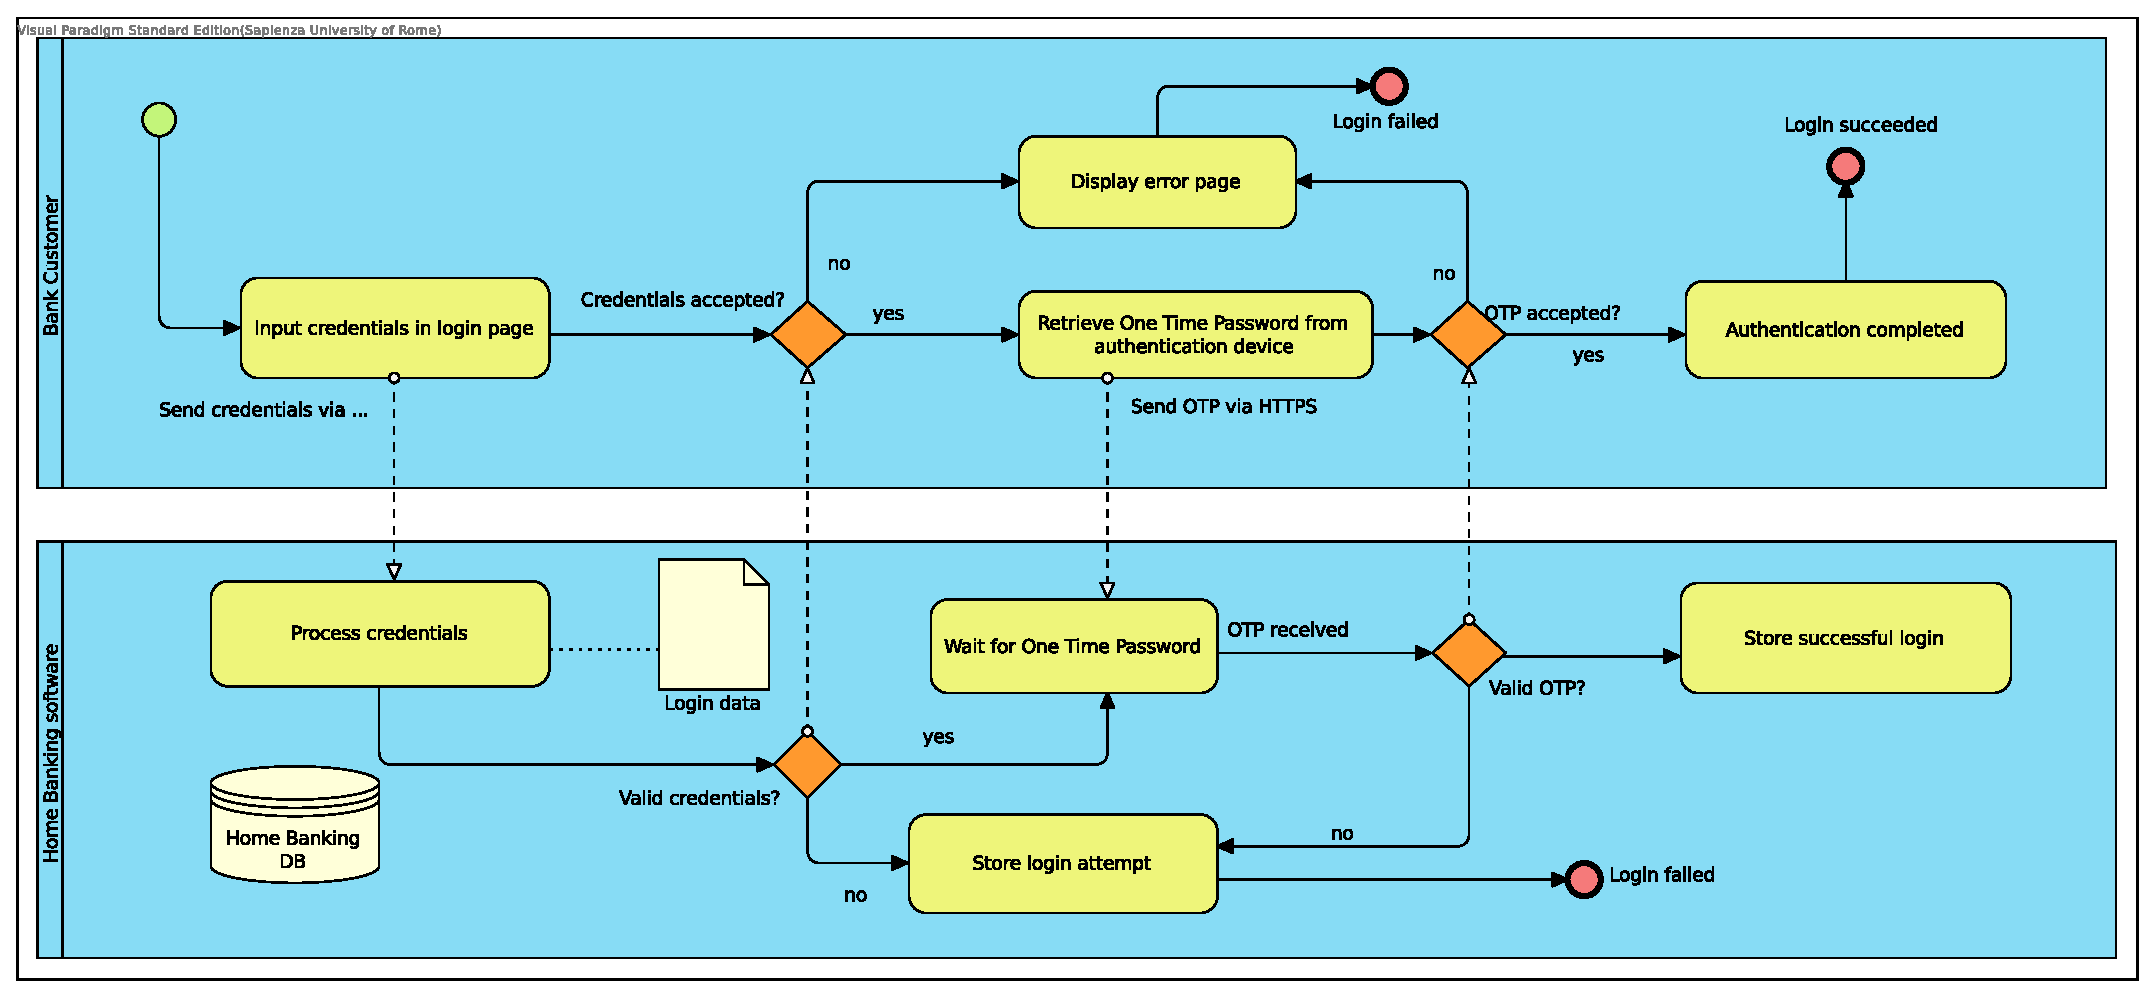
\includegraphics[width=\textheight, angle=90]{Images/Authentication.eps}
	\caption{Business case: procedura di autenticazione.}
	\label{fig:business_case_authentication}
\end{figure*}

\begin{figure*}[hbt]
	\centering
	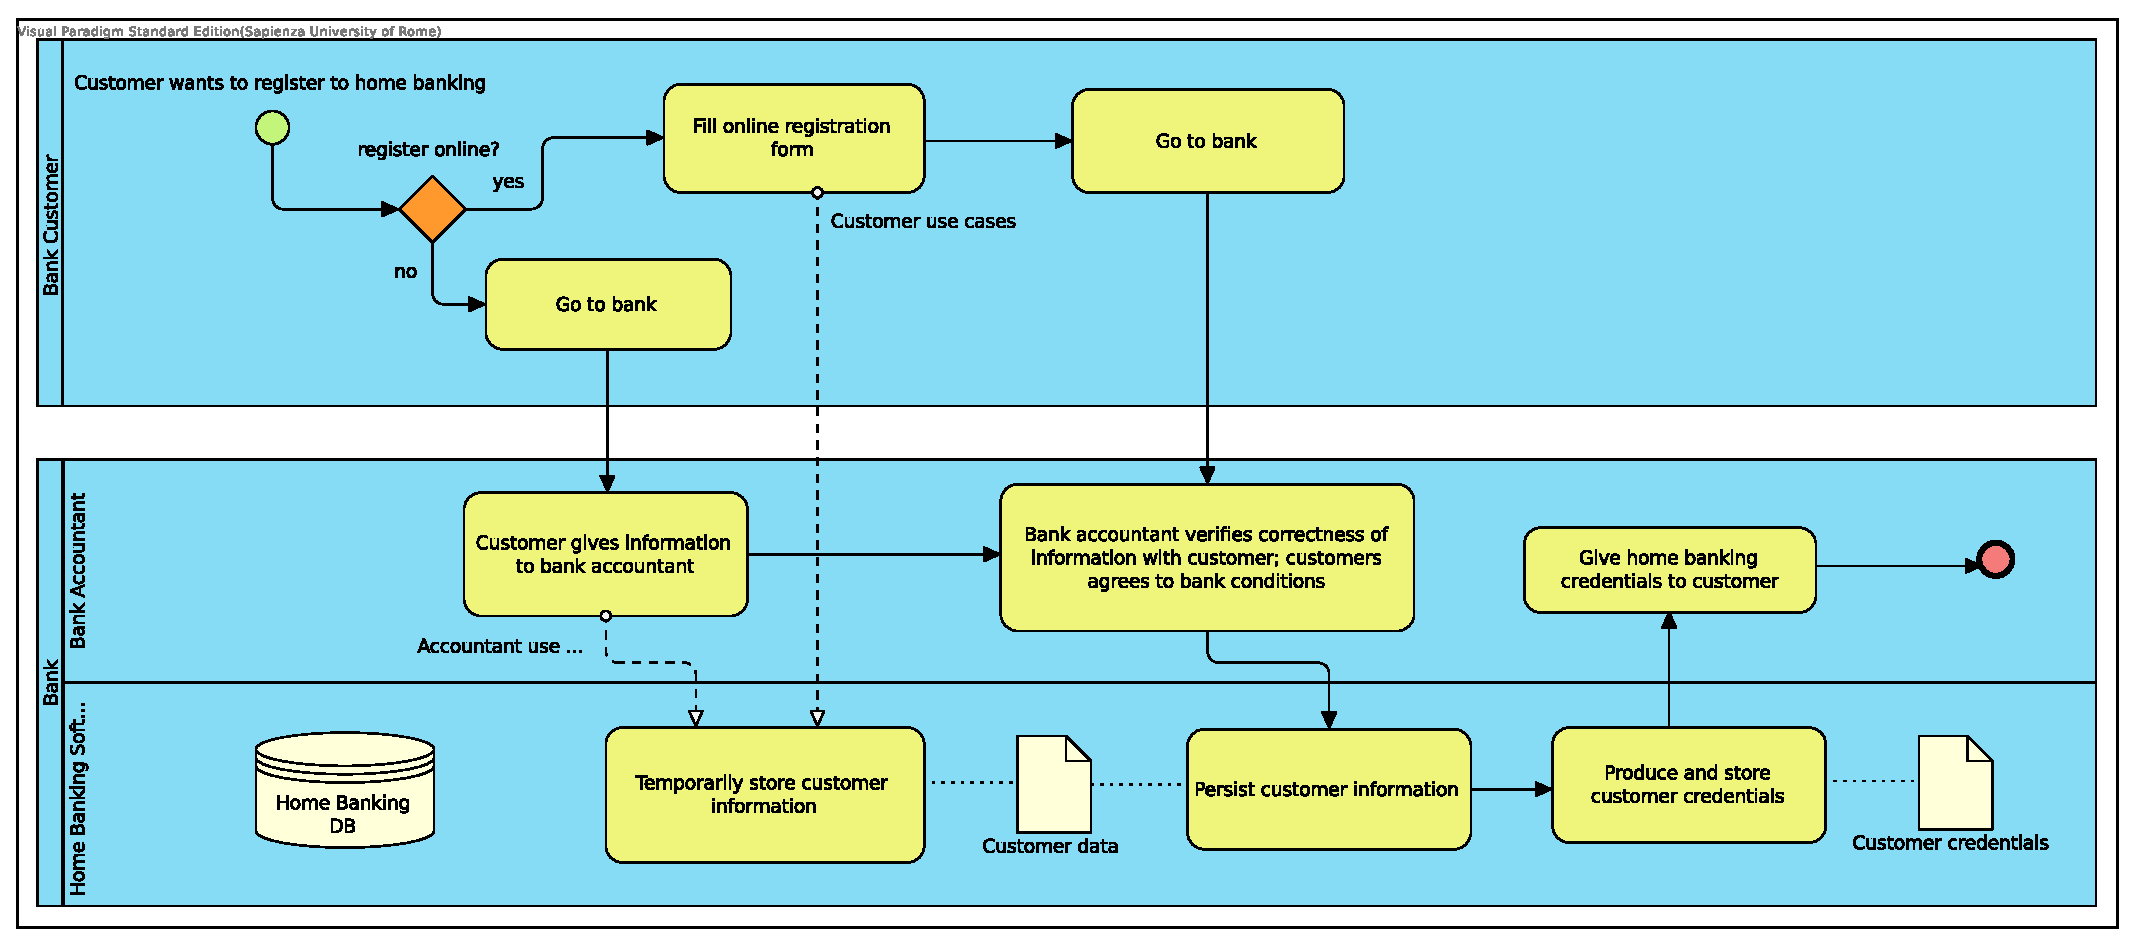
\includegraphics[width=\textheight, angle=90]{Images/Home_Banking_registration.eps}
	\caption{Business case: procedura di registrazione.}
	\label{fig:business_case_registration}
\end{figure*}

\begin{figure*}[hbt]
	\centering
	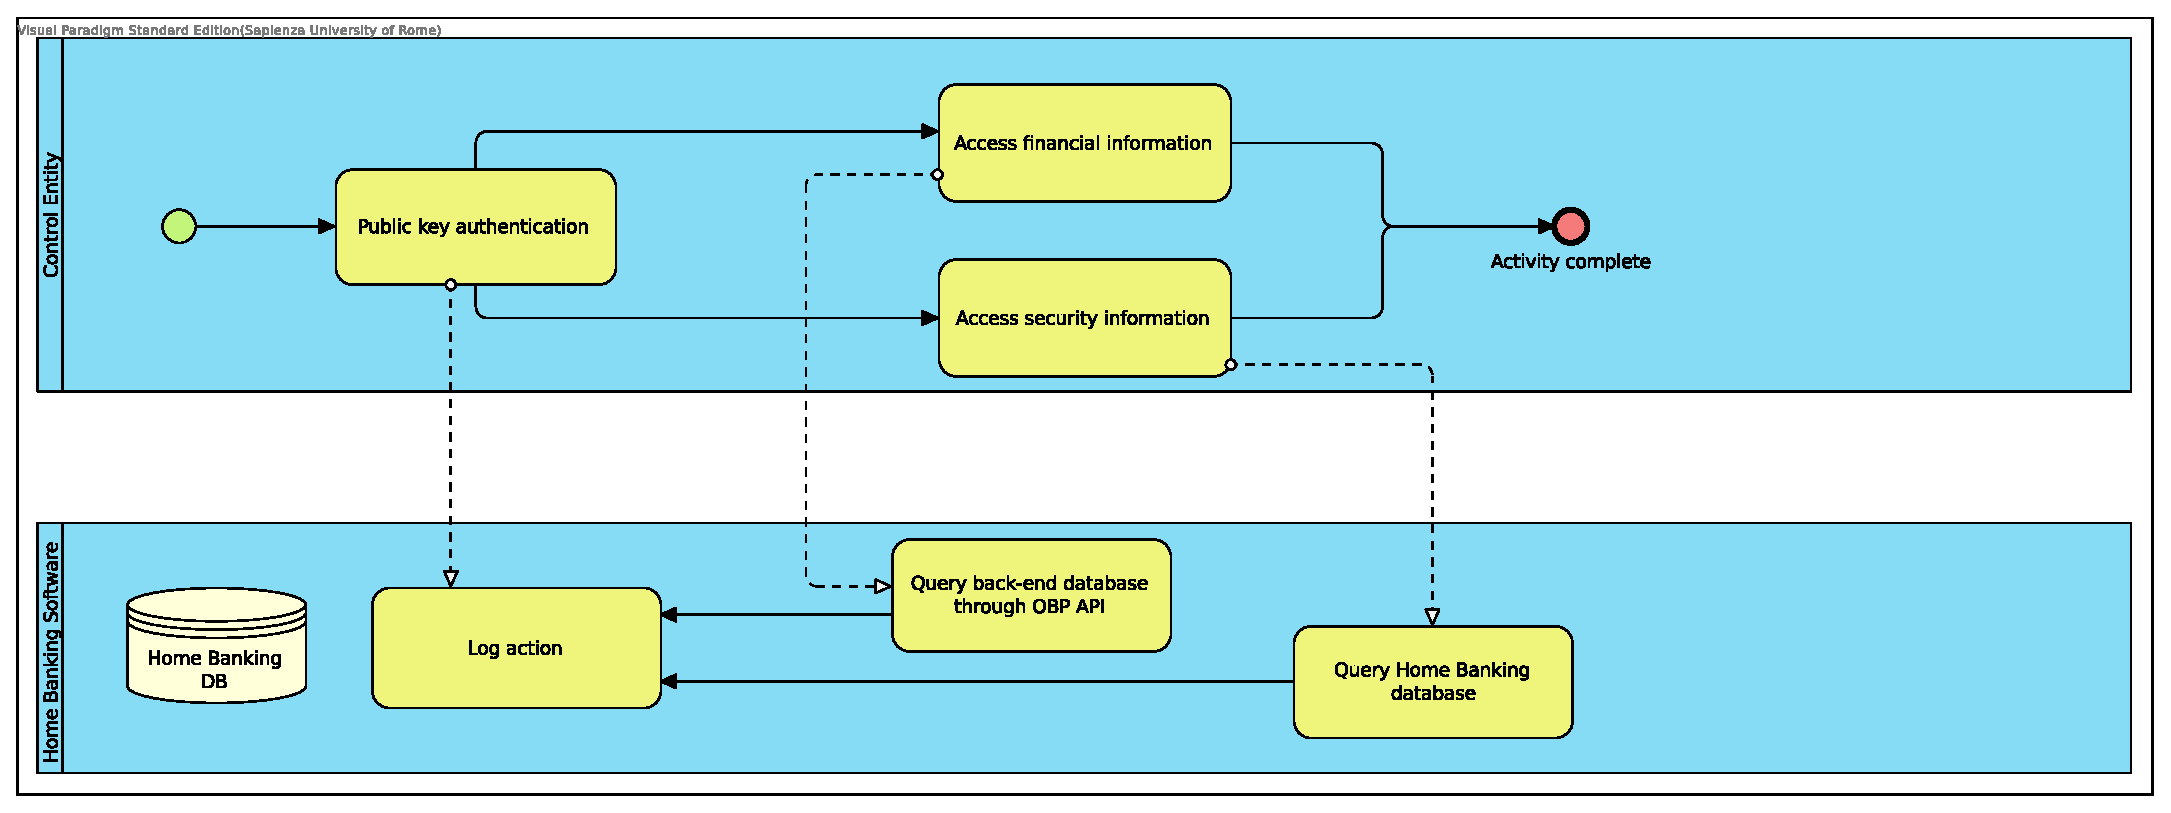
\includegraphics[width=\textheight, angle=90]{Images/Home_Banking_control_activity.eps}
	\caption{Business case: attivit\`a di controllo effettuata da enti responsabili.}
	\label{fig:business_case_control_activity}
\end{figure*}

\begin{figure*}[hbt]
	\centering
	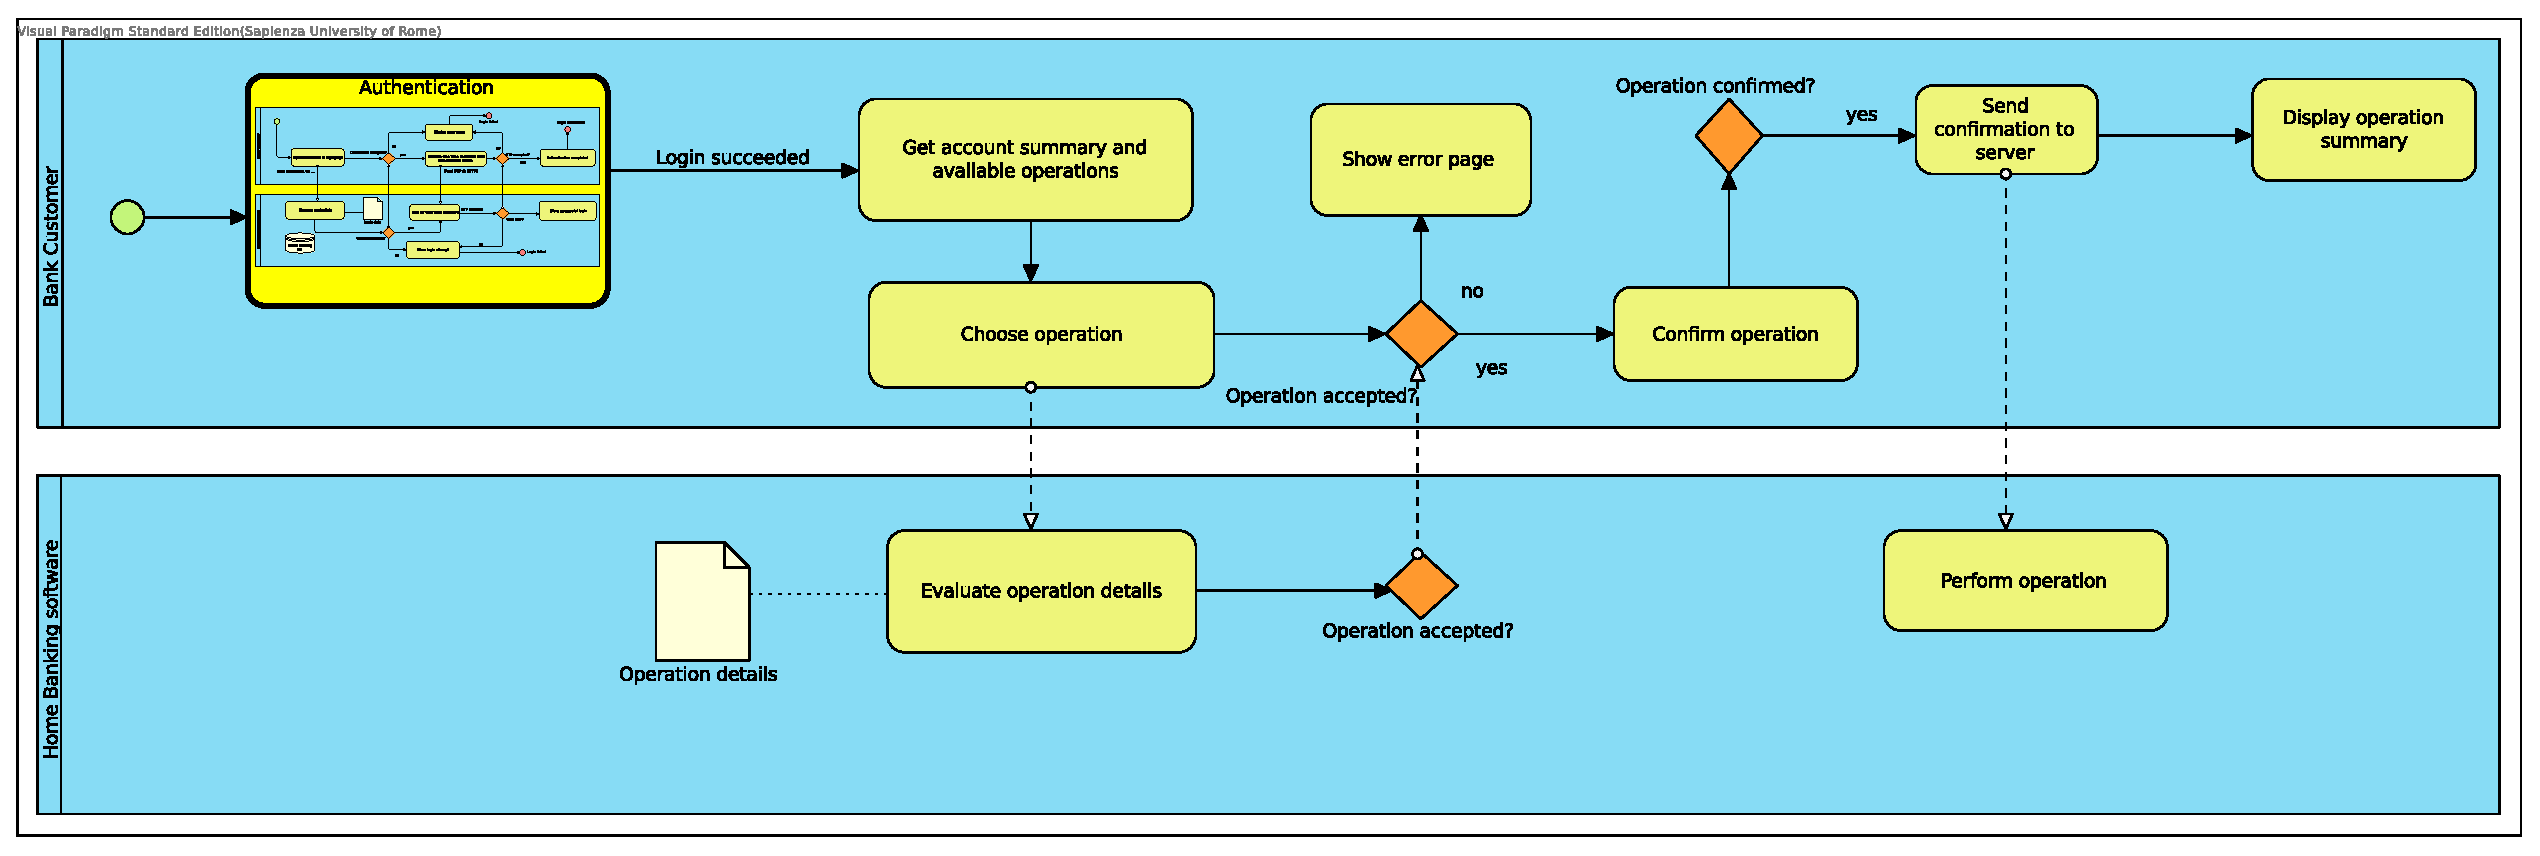
\includegraphics[width=\textheight, angle=90]{Images/Home_Banking_generic_action.eps}
	\caption{Business case: generica procedura di Home Banking effettuata da un utente del sistema.}
	\label{fig:business_case_generic_operation}
\end{figure*}

\appendix

\section{Registro Modifiche}

\subsection{Inception}

\subsubsection{I Iterazione}

Prima stesura documento.

\subsubsection{II Iterazione}

Effettuata specifica dei requisiti per fase di Inception.
Aggiunta definizione requisito funzionale di \emph{Home Trading}.
Aggiunto diagramma alto livello degli use cases del sistema.
Aggiunta possibilit\`a di effettuare bidding per mutui e prestiti.

\subsubsection{III Iterazione}

Correzione di errori.

\subsection{Elaboration}

\subsubsection{I Iterazione}

Aggiunta specifica dei requisiti di sistema.

\subsubsection{II Iterazione}

%----------------------------------------------------------------------------------------
%	REFERENCE LIST
%----------------------------------------------------------------------------------------

%\nocite{banca_italia}
\printcustombib{}

\end{document}
